\documentclass[a4paper,12pt]{article} 

% First, we usually want to set the margins of our document. For this we use the package geometry.
\usepackage[top = 2.5cm, bottom = 2.5cm, left = 2.5cm, right = 2.5cm]{geometry} 
\usepackage[T1]{fontenc}
\usepackage[utf8]{inputenc}

% The following two packages - multirow and booktabs - are needed to create nice looking tables.
\usepackage{multirow} % Multirow is for tables with multiple rows within one cell.
\usepackage{booktabs} % For even nicer tables.

% As we usually want to include some plots (.pdf files) we need a package for that.
\usepackage{graphicx} 

% The default setting of LaTeX is to indent new paragraphs. This is useful for articles. But not really nice for homework problem sets. The following command sets the indent to 0.
% \usepackage{setspace}
% \setlength{\parindent}{0in}
\usepackage{indentfirst}

% Package to place figures where you want them.
\usepackage{float}

% The fancyhdr package let's us create nice headers.
\usepackage{fancyhdr}

\usepackage{amsmath,amsthm}
\usepackage{minted}

\begin{document}

\section{Ports of the Decoder module}

\begin{table}[H]
	\begin{center}
		\begin{tabular}{ccccc}
			\toprule
			Port Name & From & To & Bit Width & Description \\
			\midrule
			\texttt{clk} & Clock signal generator & Decoder & 1 & clock signal \\
			\texttt{rst\_n} & Reset button & Decoder & 1 & reset all registers (active low) \\
			\texttt{inst} & IFetch & Decoder & 32 & instruction \\
			\texttt{read\_reg\_1} & IFetch & Decoder & 5 & first register to read \\
			\texttt{read\_reg\_2} & IFetch & Decoder & 5 & second register to read \\
			\texttt{write\_reg} & IFetch & Decoder & 5 & register to write \\
			\texttt{write\_data} & Memory & Decoder & 32 & data to write \\
			\texttt{write\_reg\_flag} & Control & Decoder & 1 & flag to write register \\
			\hline
			\texttt{read\_data\_1} & Decoder & ALU & 32 & data in \texttt{read\_reg\_1} \\
			\texttt{read\_data\_2} & Decoder & ALU & 32 & data in \texttt{read\_reg\_2} \\
			\texttt{imme} & Decoder & ALU & 32 & immediate value from \texttt{inst} \\
			\bottomrule
			
		\end{tabular}
	\end{center}
	\caption{Ports of the Decoder module}
\end{table}

\section{Testbench for the Decoder module}

\begin{figure}[H]
	\centering
	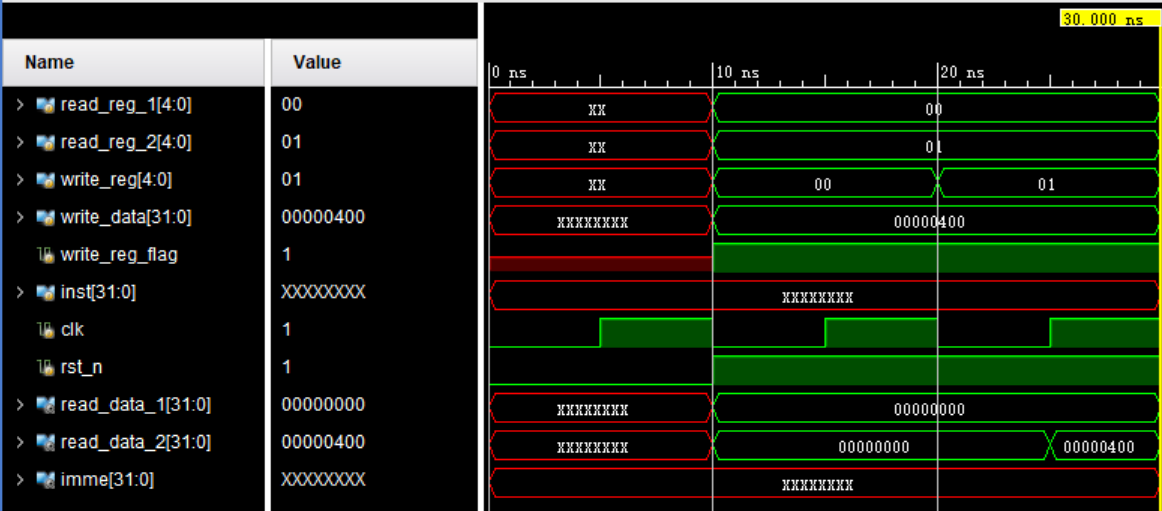
\includegraphics[width=\textwidth]{decoder1.png}
	\caption{Testbench 1}
\end{figure}

This testbench tests the following cases:
\begin{enumerate}
	\item Register \texttt{x0} cannot be written.
	\item Register \texttt{x1} is correctly written.
	\item Register \texttt{x0} and \texttt{x1} are correctly read.
	\item Register write operation only occurs on the positive edge of the clock signal.
\end{enumerate}

\begin{figure}[H]
	\centering
	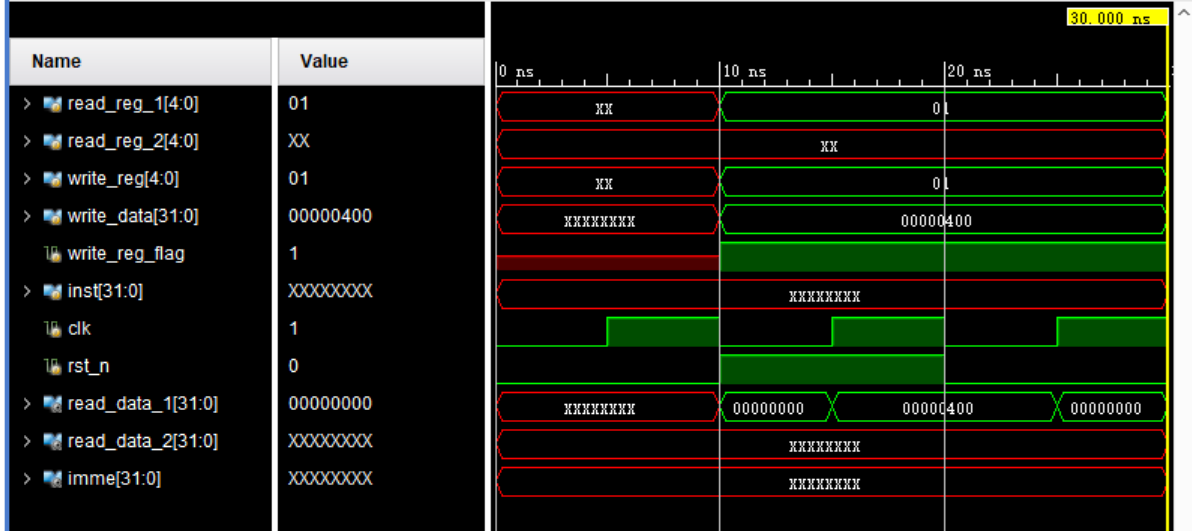
\includegraphics[width=\textwidth]{decoder2.png}
	\caption{Testbench 2}
\end{figure}

This testbench tests the following cases:
\begin{enumerate}
	\item \texttt{rst\_n} signal resets all registers (happen on the positive edge of the clock signal).
	\item \texttt{rst\_n} signal overrides the writing operation of the register.
\end{enumerate}

\begin{figure}[H]
	\centering
	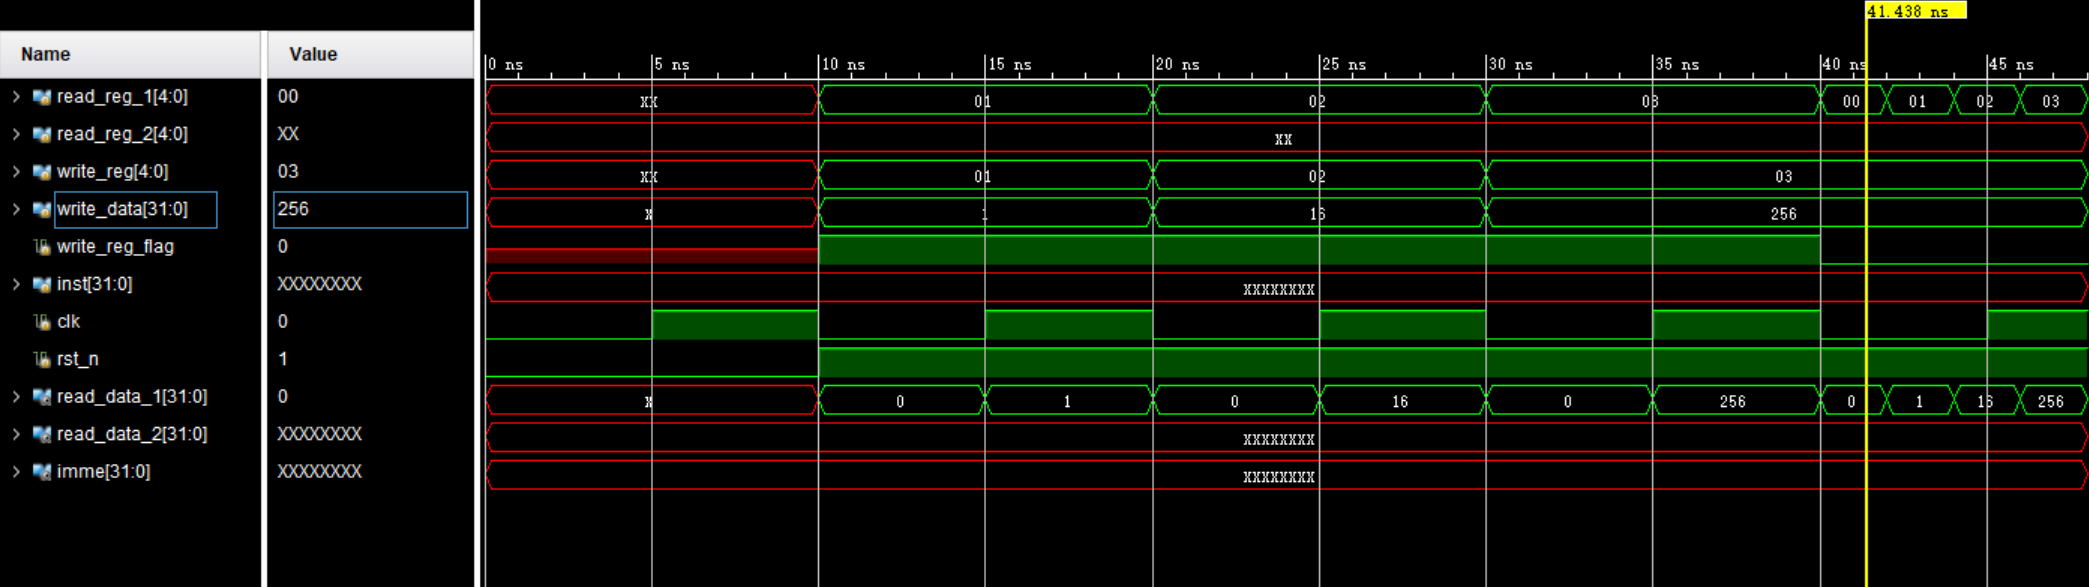
\includegraphics[width=\textwidth]{decoder3.png}
	\caption{Testbench 3}
\end{figure}

This testbench tests the following cases:
\begin{enumerate}
	\item The reading operation of the register can occur at any time (last 8ms of the simulation).
\end{enumerate}

The immediate extraction is tested last week and is not included in this testbench.

\section{Code for the Decoder module}

\begin{center}
	\begin{minted}{verilog}
`timescale 1ns / 1ps

module decoder(
input [4:0] read_reg_1,
input [4:0] read_reg_2,
input [4:0] write_reg,
input [31:0] write_data,
input write_reg_flag,
input [31:0] inst,
input clk,
input rst_n,
output [31:0] read_data_1,
output [31:0] read_data_2,
output [31:0] imme
);

immediate_generator imme_gen(.inst(inst), .imme(imme));

reg [31:0] register [0:31];
assign read_data_1 = register[read_reg_1];
assign read_data_2 = register[read_reg_2];
    
always @(posedge clk)
begin
    if(!rst_n)
    begin
        register[0] <= 32'b0;
        register[1] <= 32'b0;
        register[2] <= 32'b0;
        register[3] <= 32'b0;
        register[4] <= 32'b0;
        register[5] <= 32'b0;
        register[6] <= 32'b0;
        register[7] <= 32'b0;
        register[8] <= 32'b0;
        register[9] <= 32'b0;
        register[10] <= 32'b0;
        register[11] <= 32'b0;
        register[12] <= 32'b0;
        register[13] <= 32'b0;
        register[14] <= 32'b0;
        register[15] <= 32'b0;
        register[16] <= 32'b0;
        register[17] <= 32'b0;
        register[18] <= 32'b0;
        register[19] <= 32'b0;
        register[20] <= 32'b0;
        register[21] <= 32'b0;
        register[22] <= 32'b0;
        register[23] <= 32'b0;
        register[24] <= 32'b0;
        register[25] <= 32'b0;
        register[26] <= 32'b0;
        register[27] <= 32'b0;
        register[28] <= 32'b0;
        register[29] <= 32'b0;
        register[30] <= 32'b0;
        register[31] <= 32'b0;
    end else begin
        if(write_reg_flag && write_reg != 0)
        begin
            register[write_reg] <= write_data;
        end
    end
end


endmodule
	\end{minted}
\end{center}
\end{document}